% Created 2023-02-14 Tue 19:52
\documentclass[9pt, b5paper]{article}
\usepackage{xeCJK}
\usepackage[T1]{fontenc}
\usepackage{bera}
\usepackage[scaled]{beraserif}
\usepackage[scaled]{berasans}
\usepackage[scaled]{beramono}
\usepackage[cache=false]{minted}
\usepackage{xltxtra}
\usepackage{graphicx}
\usepackage{xcolor}
\usepackage{multirow}
\usepackage{multicol}
\usepackage{float}
\usepackage{textcomp}
\usepackage{algorithm}
\usepackage{algorithmic}
\usepackage{latexsym}
\usepackage{natbib}
\usepackage{geometry}
\geometry{left=1.2cm,right=1.2cm,top=1.5cm,bottom=1.2cm}
\usepackage[xetex,colorlinks=true,CJKbookmarks=true,linkcolor=blue,urlcolor=blue,menucolor=blue]{hyperref}
\newminted{common-lisp}{fontsize=\footnotesize} 
\author{deepwaterooo}
\date{\today}
\title{Emacs Configuration}
\hypersetup{
  pdfkeywords={},
  pdfsubject={},
  pdfcreator={Emacs 27.1 (Org mode 8.2.7c)}}
\begin{document}

\maketitle
\tableofcontents


\section{Updates}
\label{sec-1}
\subsection{{\bfseries\sffamily emacs} 1 initiliation bug}
\label{sec-1-1}
\begin{itemize}
\item emacs 27.1 for emacs-rime input methods. one bug to be fixed.
\end{itemize}

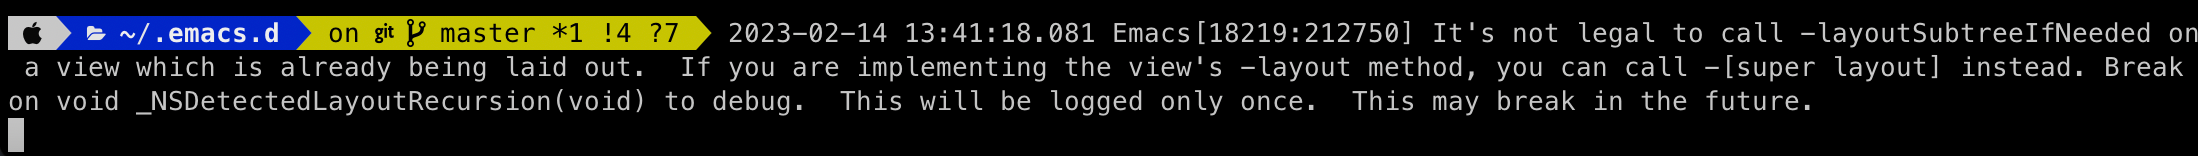
\includegraphics[width=.9\linewidth]{./pic/readme_20230214_134351.png}
\begin{itemize}
\item this affect me access to current terminal, needs to be fixed later.
\end{itemize}
\subsection{configue pyim wubi input method emacs-rime, works like a charm!}
\label{sec-1-2}
\begin{itemize}
\item emacs-rime rime 在emacs 里的前端,想要把它配置好:不能自动上屏的五笔输入法显然是太笨了.现在好了,终于有可以自动上屏的五笔输入法了
\end{itemize}
\subsection{configuration for pdf-tools packages}
\label{sec-1-3}

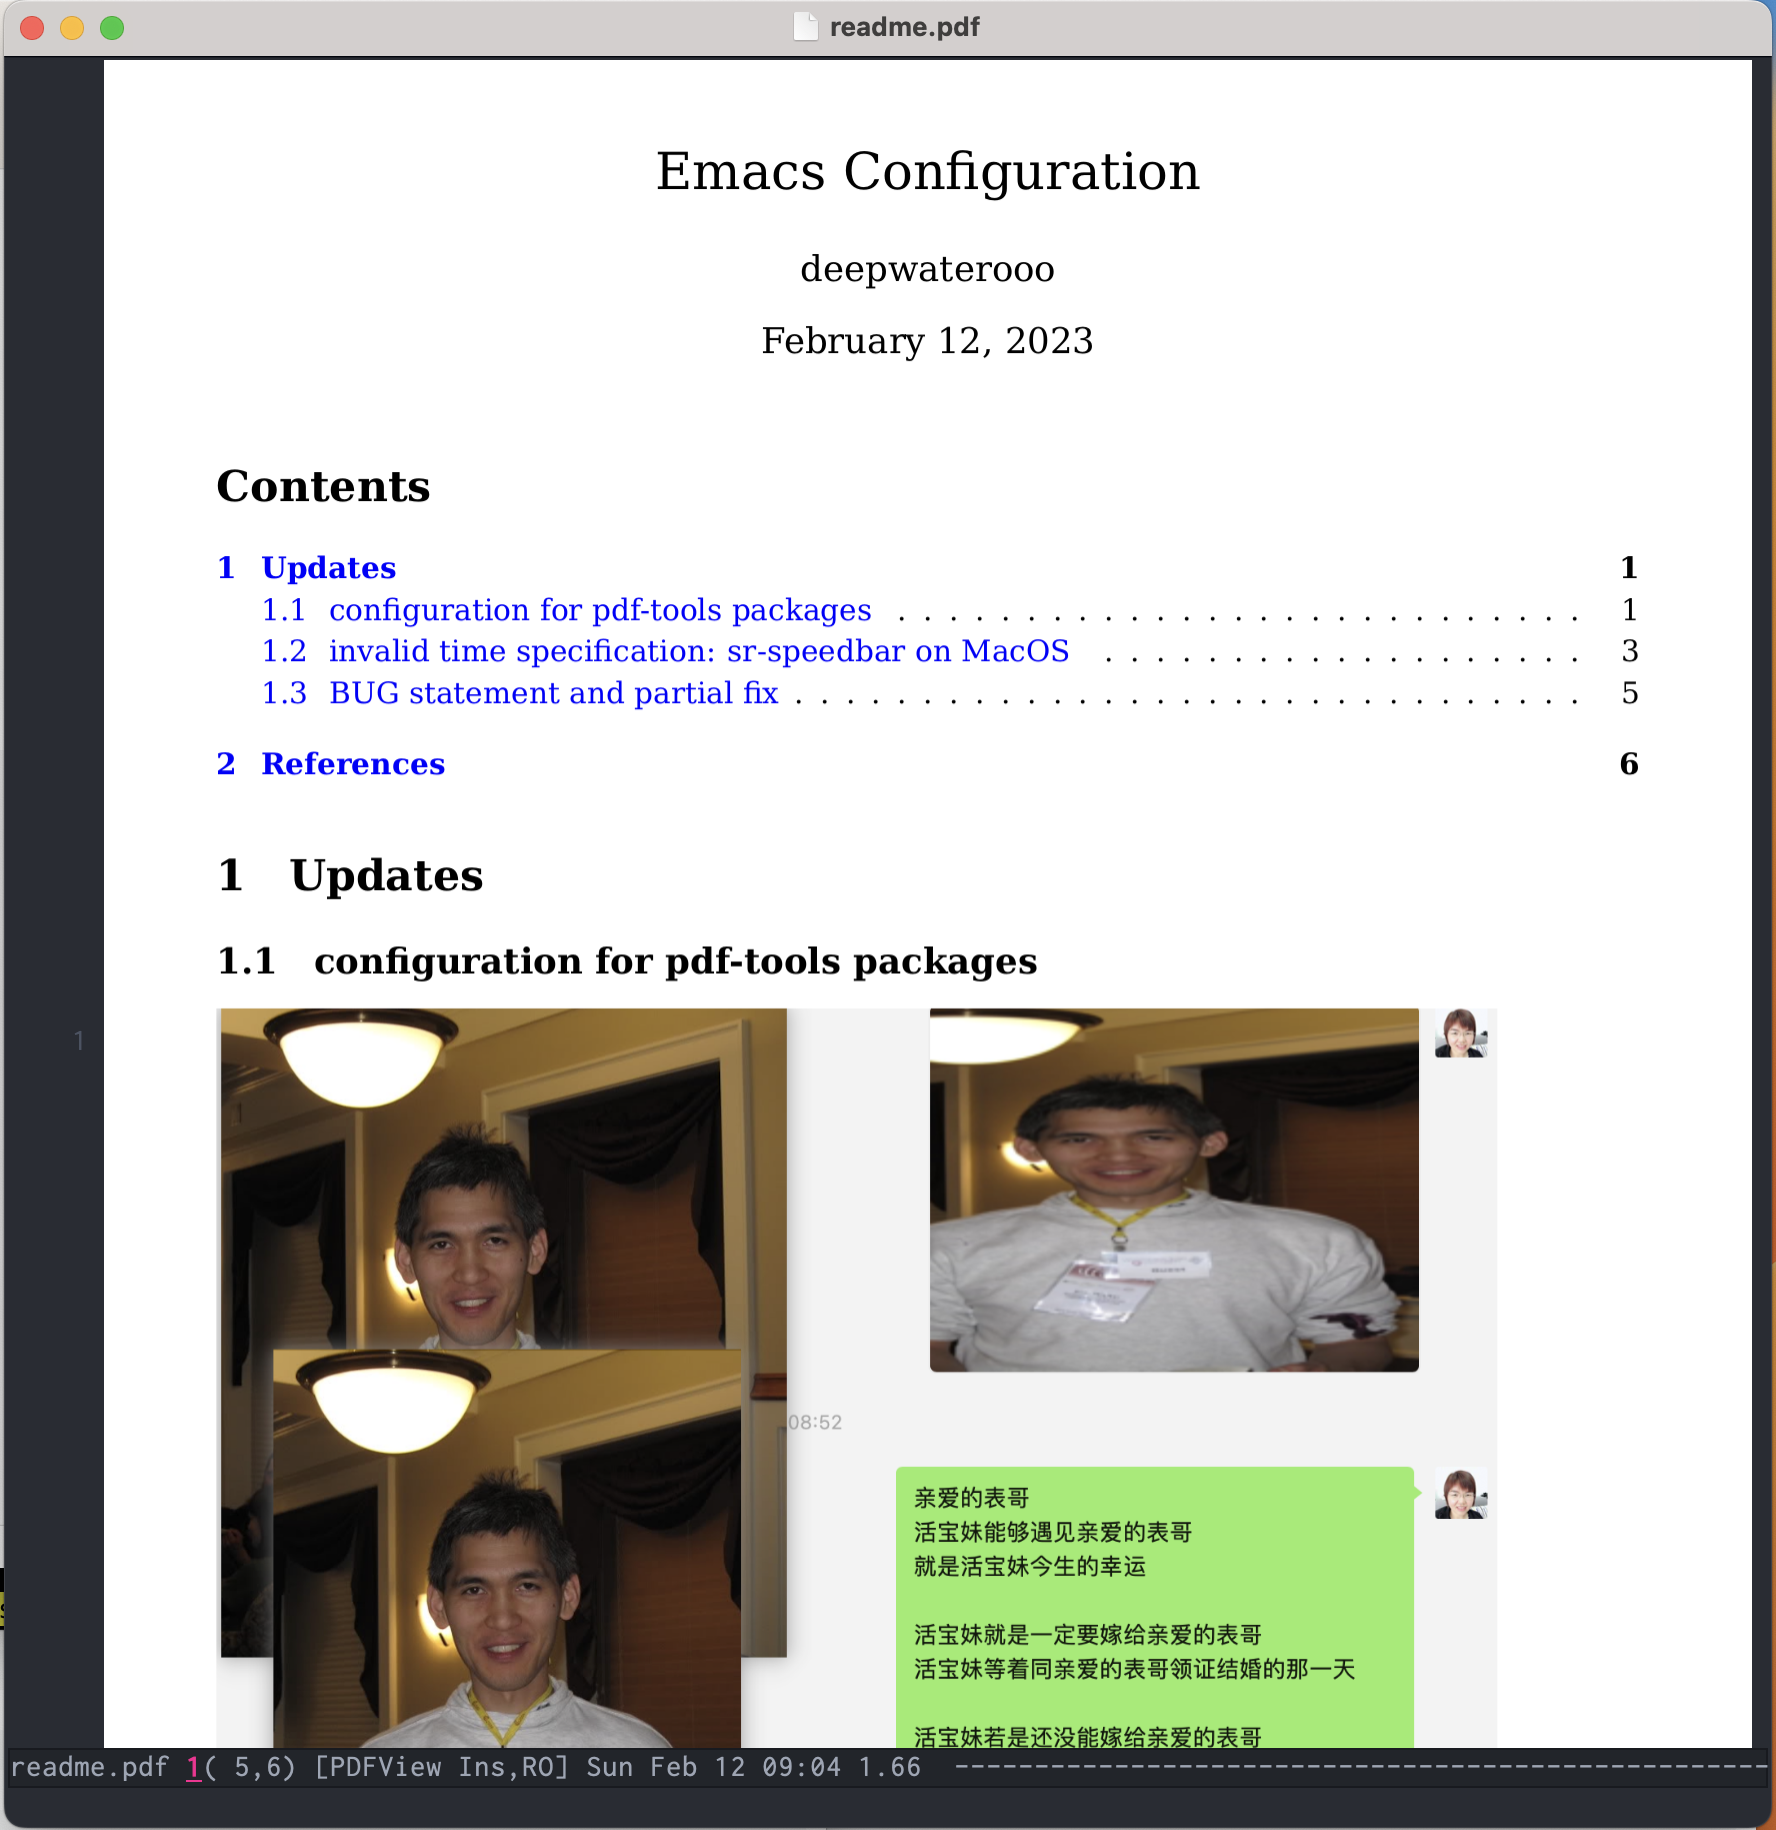
\includegraphics[width=.9\linewidth]{./pic/mememe2.png}

\begin{itemize}
\item pdf viewer noter <==> Skim bi-directional linking configuration on the way, most emacs work is done. Need to learn how to use them though.
\end{itemize}

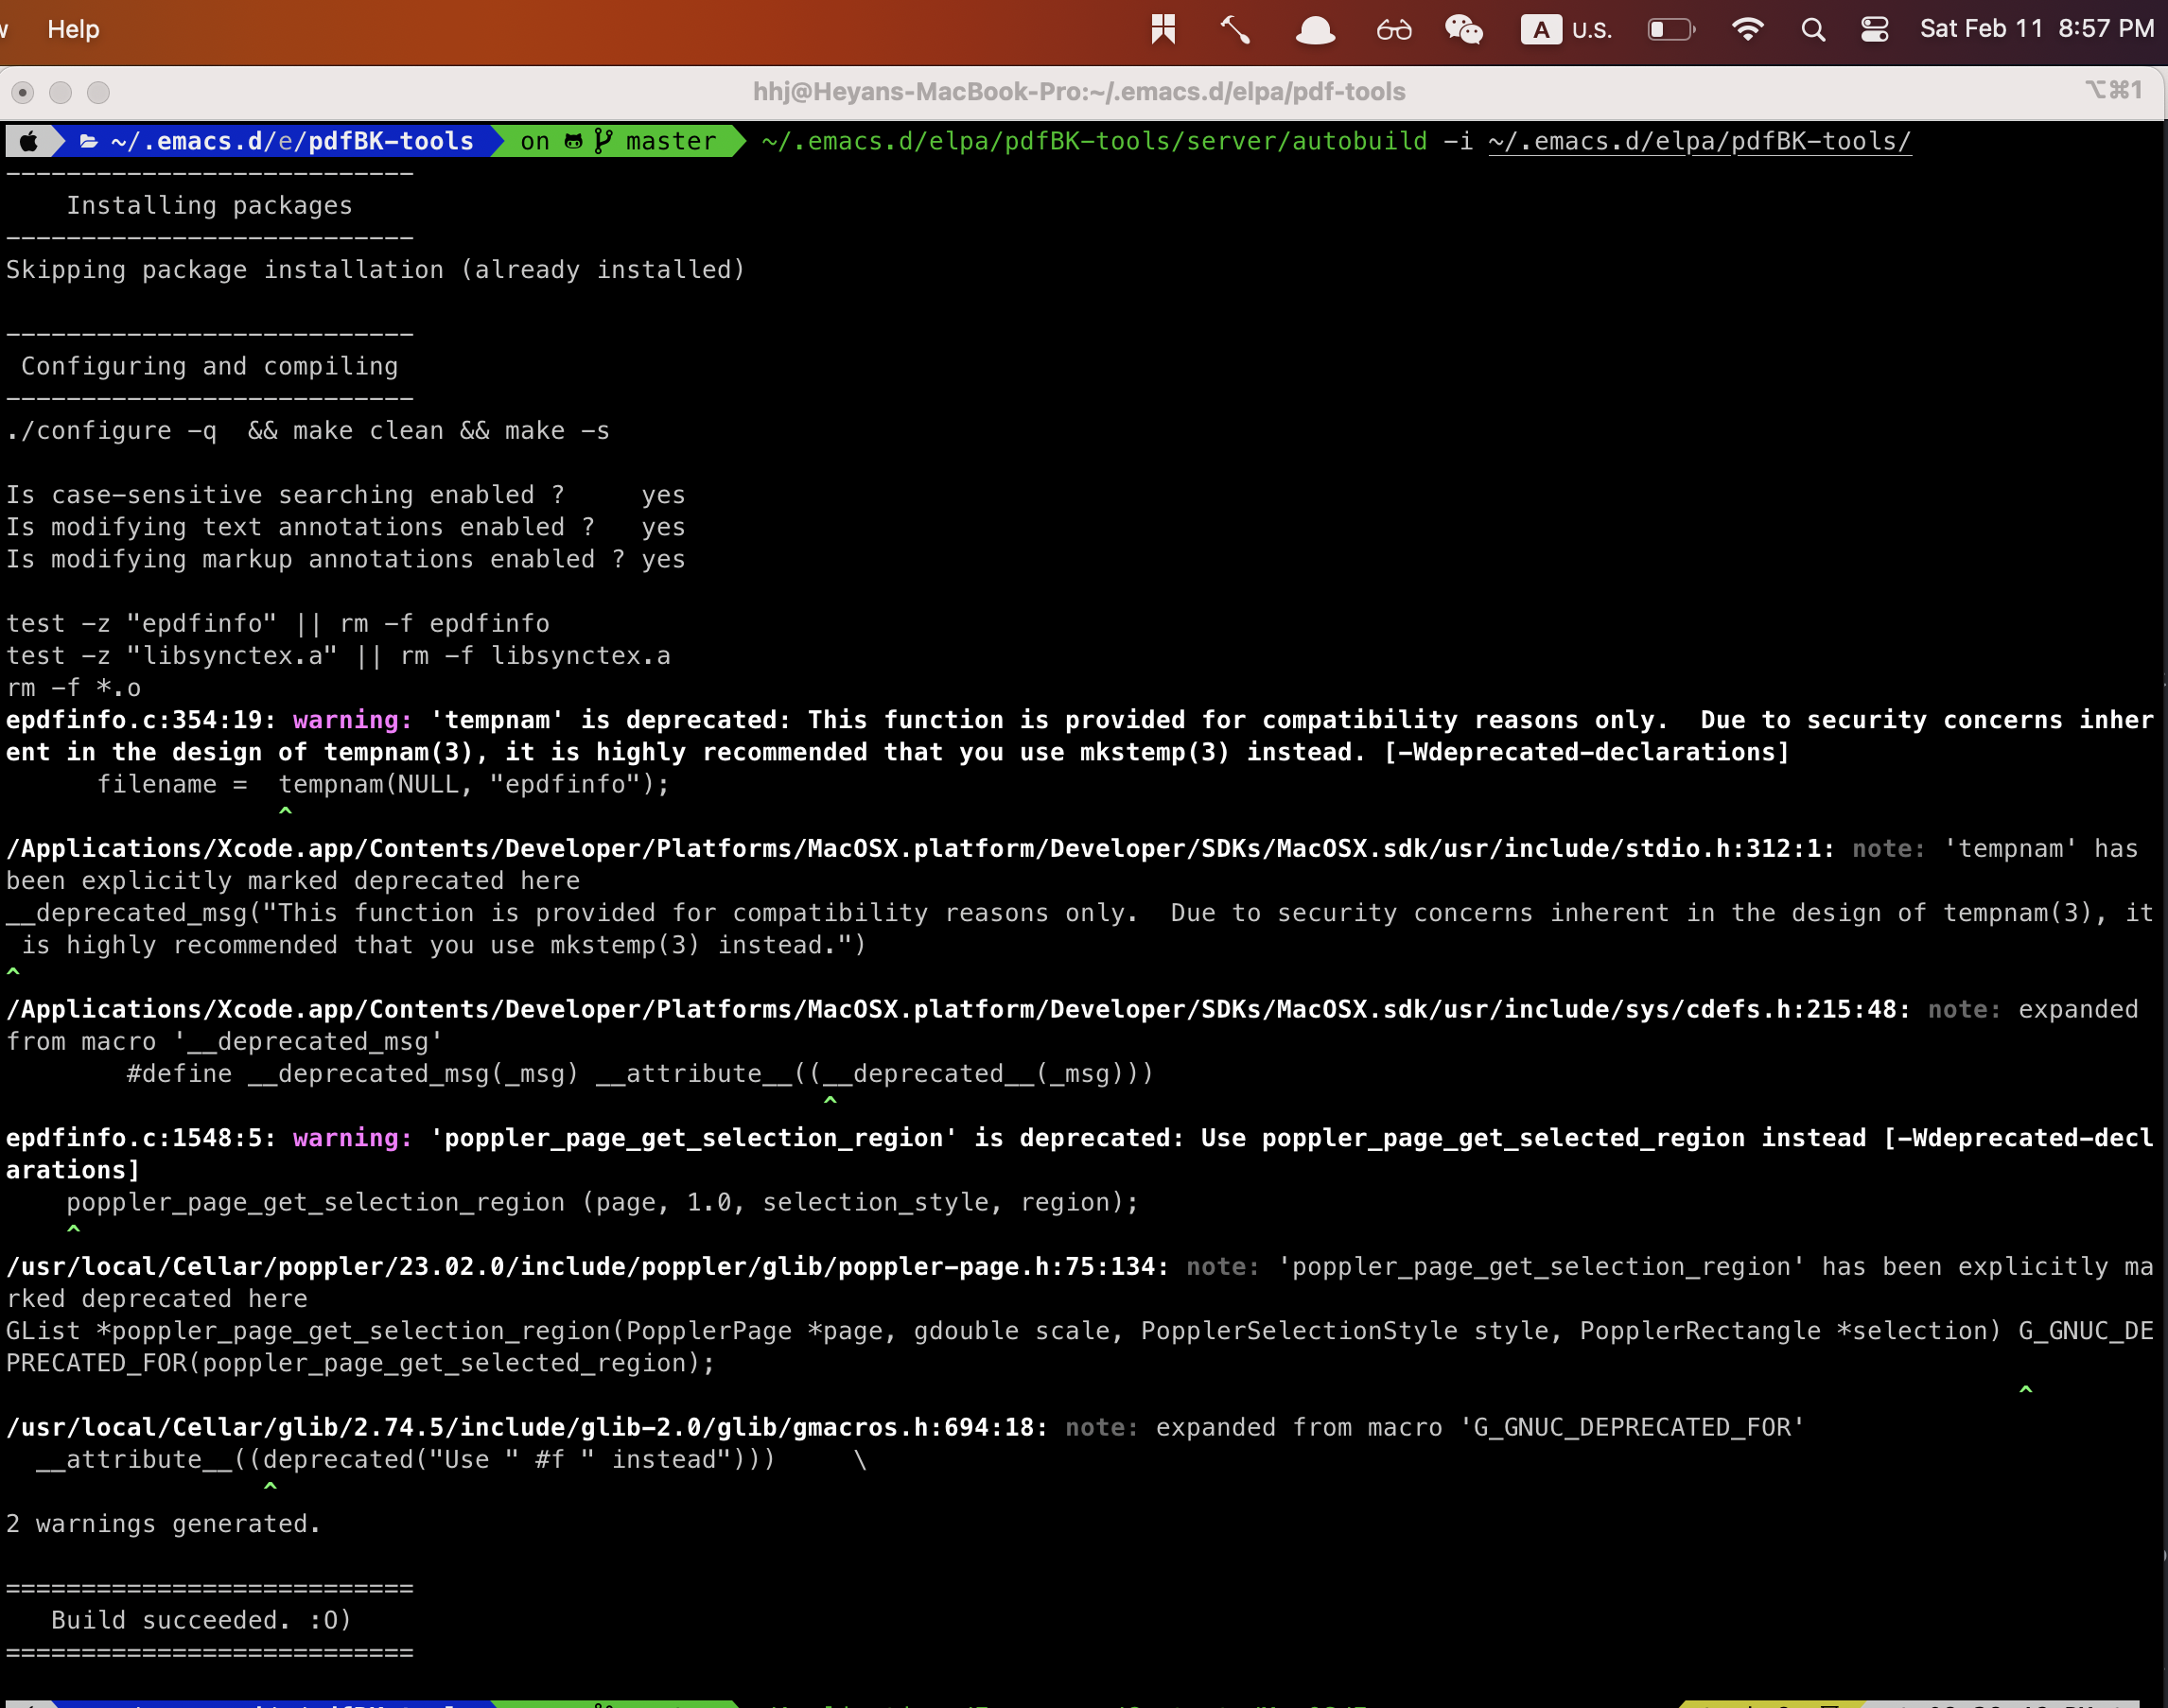
\includegraphics[width=.9\linewidth]{./pic/Snipaste_2023-02-11_20-57-40.png}
\begin{itemize}
\item It has to be configured for M1. But I am still not getting any .tar file yet. 

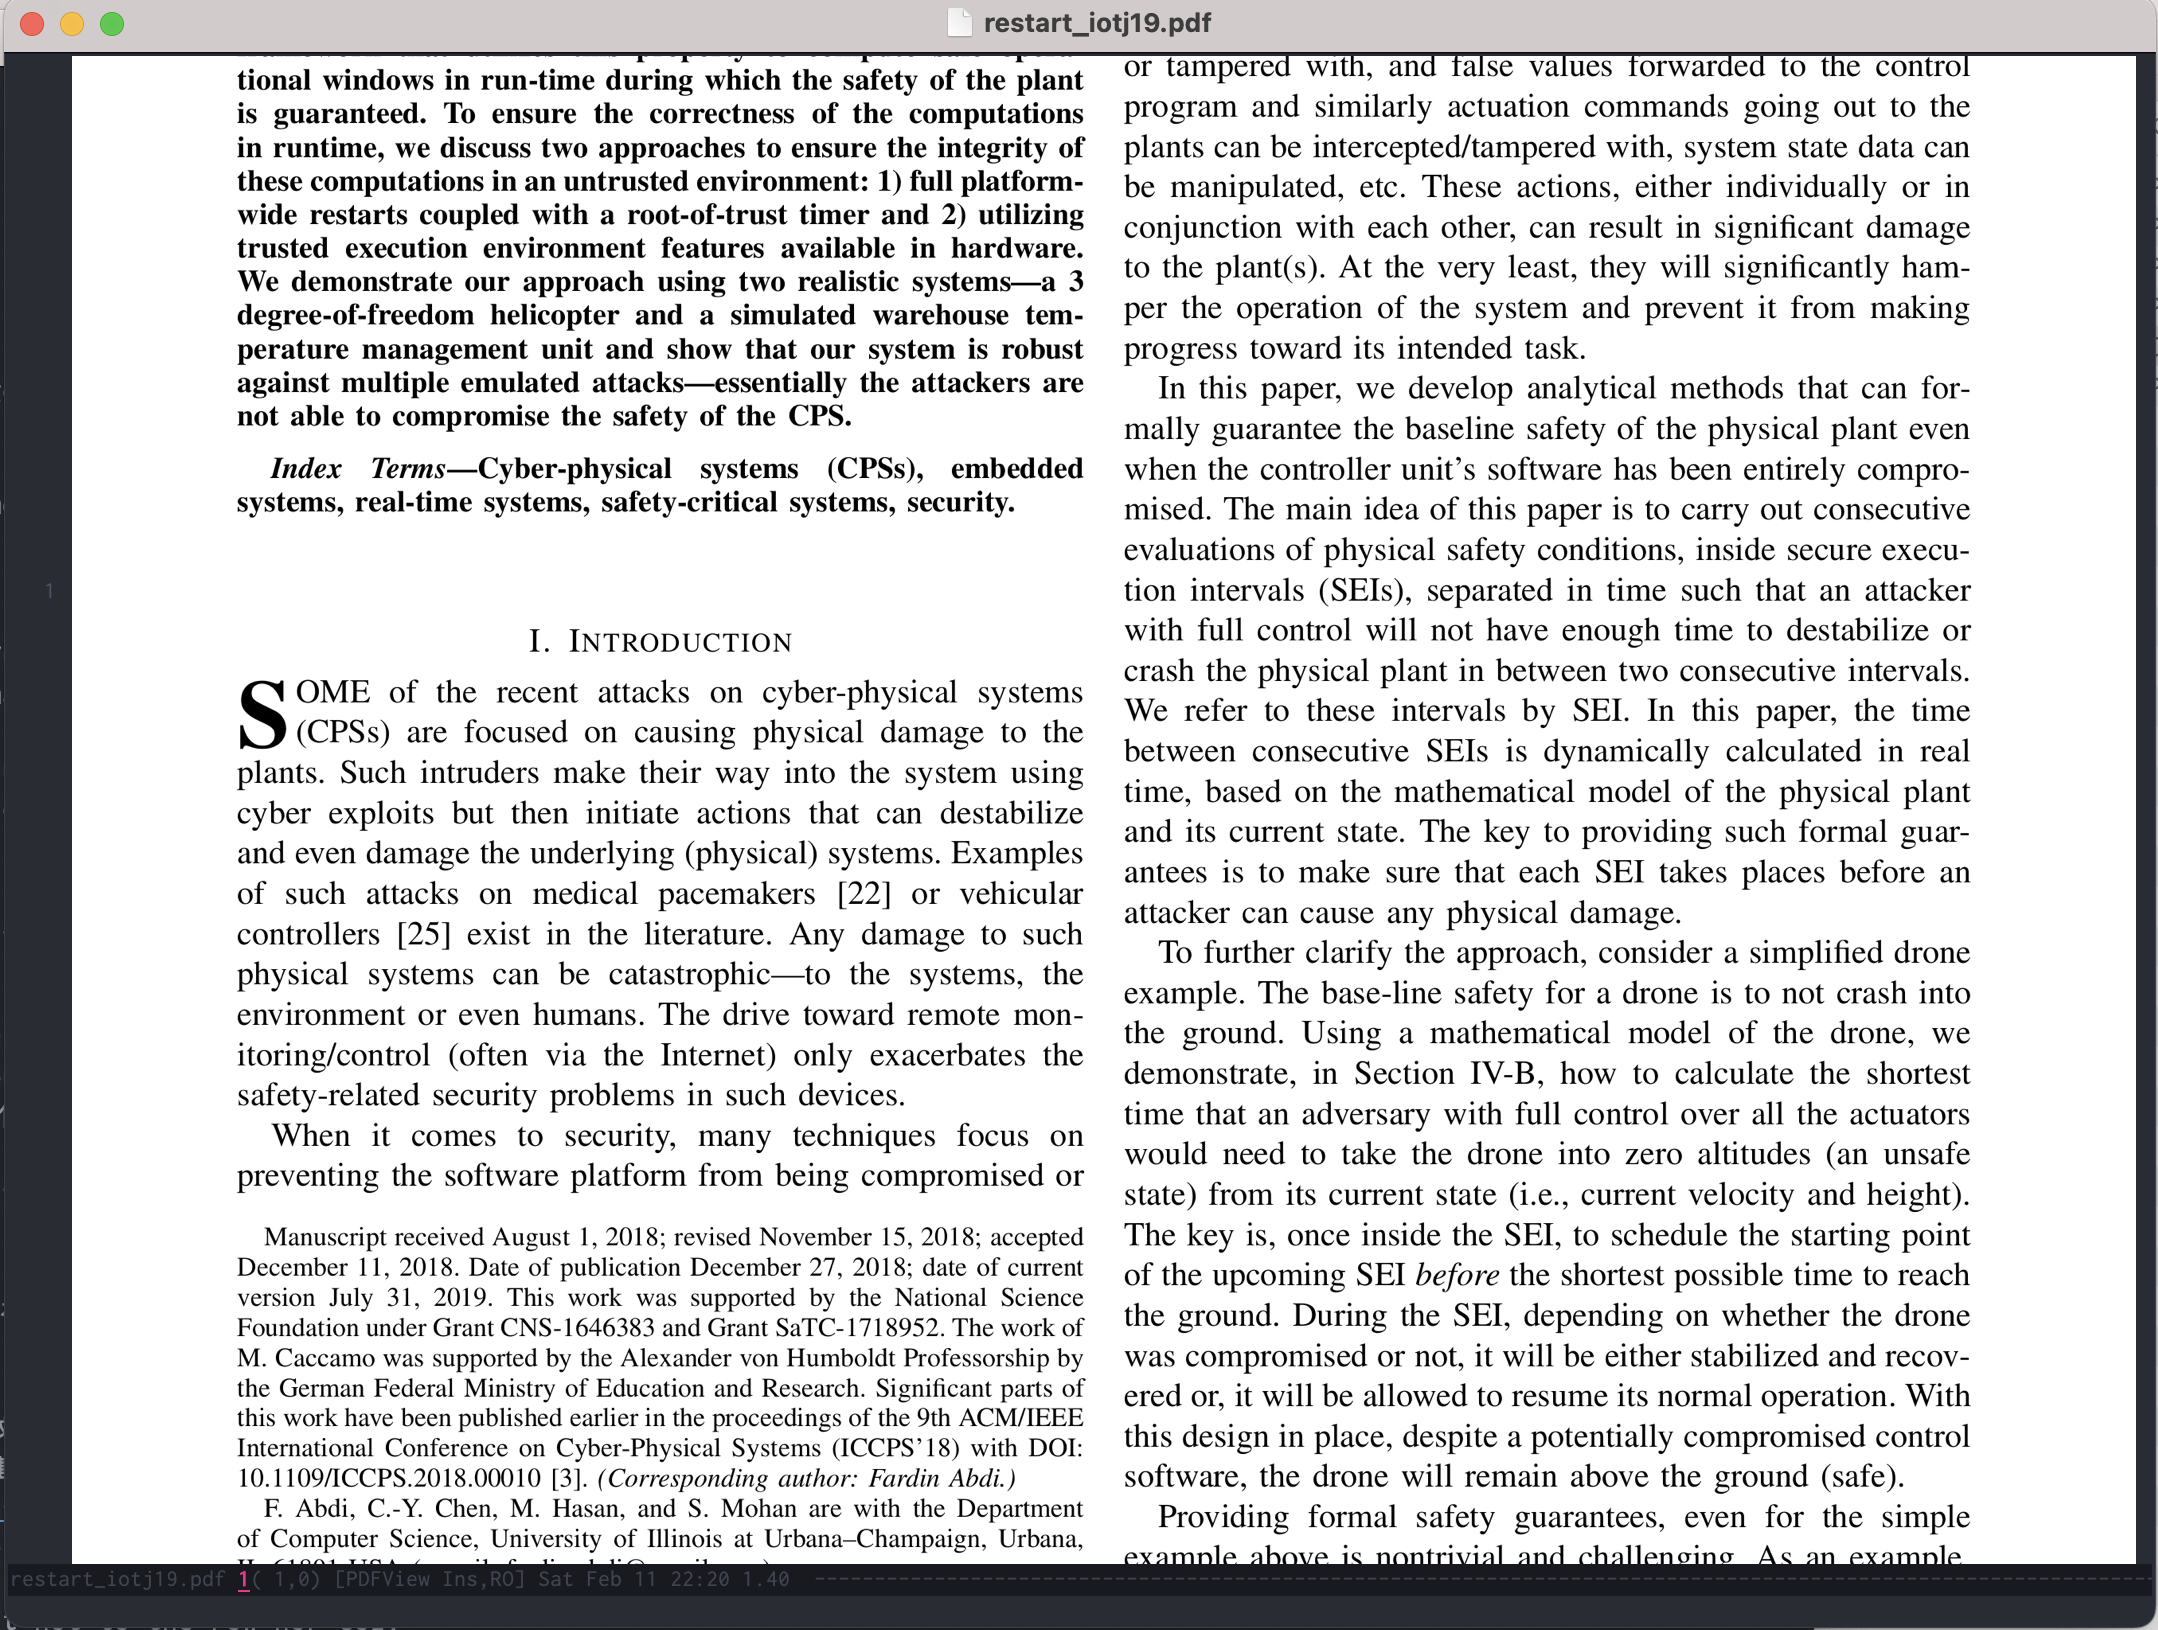
\includegraphics[width=.9\linewidth]{./pic/Snipaste_2023-02-11_22-20-25.png}
\item could customer F5 toggle sr-speedbar, and make sis-mode work. But I do NOT really need sis-mode, only needed macism command line. to help [LOVE MY DEAR COUSIN!!!]
\end{itemize}

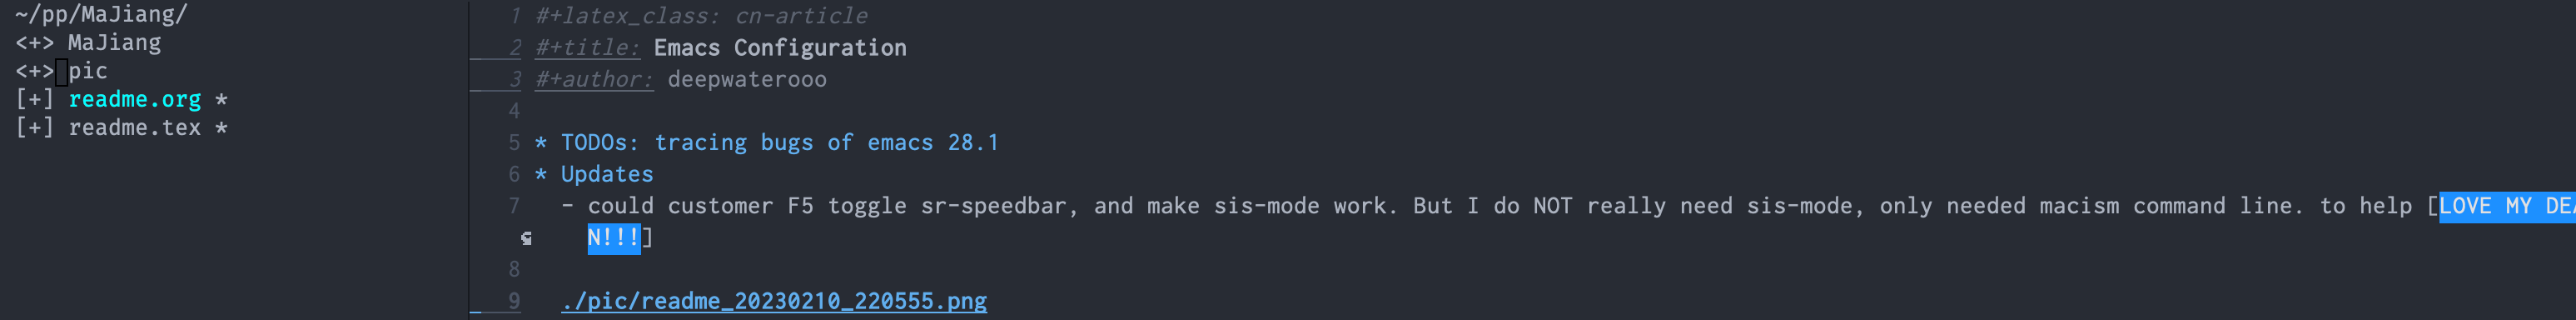
\includegraphics[width=.9\linewidth]{./pic/readme_20230210_221127.png}
\begin{itemize}
\item finally sync up with csharp-mode with tree-sitter, and fixed added the other's that gio-mode etc.
\item Permanently diabled speedbar-edit-file's set-timer function call from Resource files. Do NOT want to see such a bug, don't know how to fix, but disable it and walk around.
\item Now have a relatively barable and stable colorful emacs code editor now, at least for csharp-mode. Relatively satisfied now. Could sit it aside for a while now to focus on projects.
\end{itemize}
\subsection{invalid time specification: sr-speedbar on MacOS}
\label{sec-1-4}
\begin{itemize}
\item I don't like this bug, and I belive I do NOT really using any timer for auto-refresh in my speedbar. So I ended up by disabling the (speedbar-edit-file() func, which is frequently bug trigered) setting timer part from /Applications/Emacs.app/Contents/Resources/lisp/speedbar.el.gz, and recompile the file. The bug was gone. And I could deal with csharp-mode's fontify bug.
\item newer debugging infos, concernibg about sr-speedbar.el file. Have NOT been able to trace down for today.
\end{itemize}

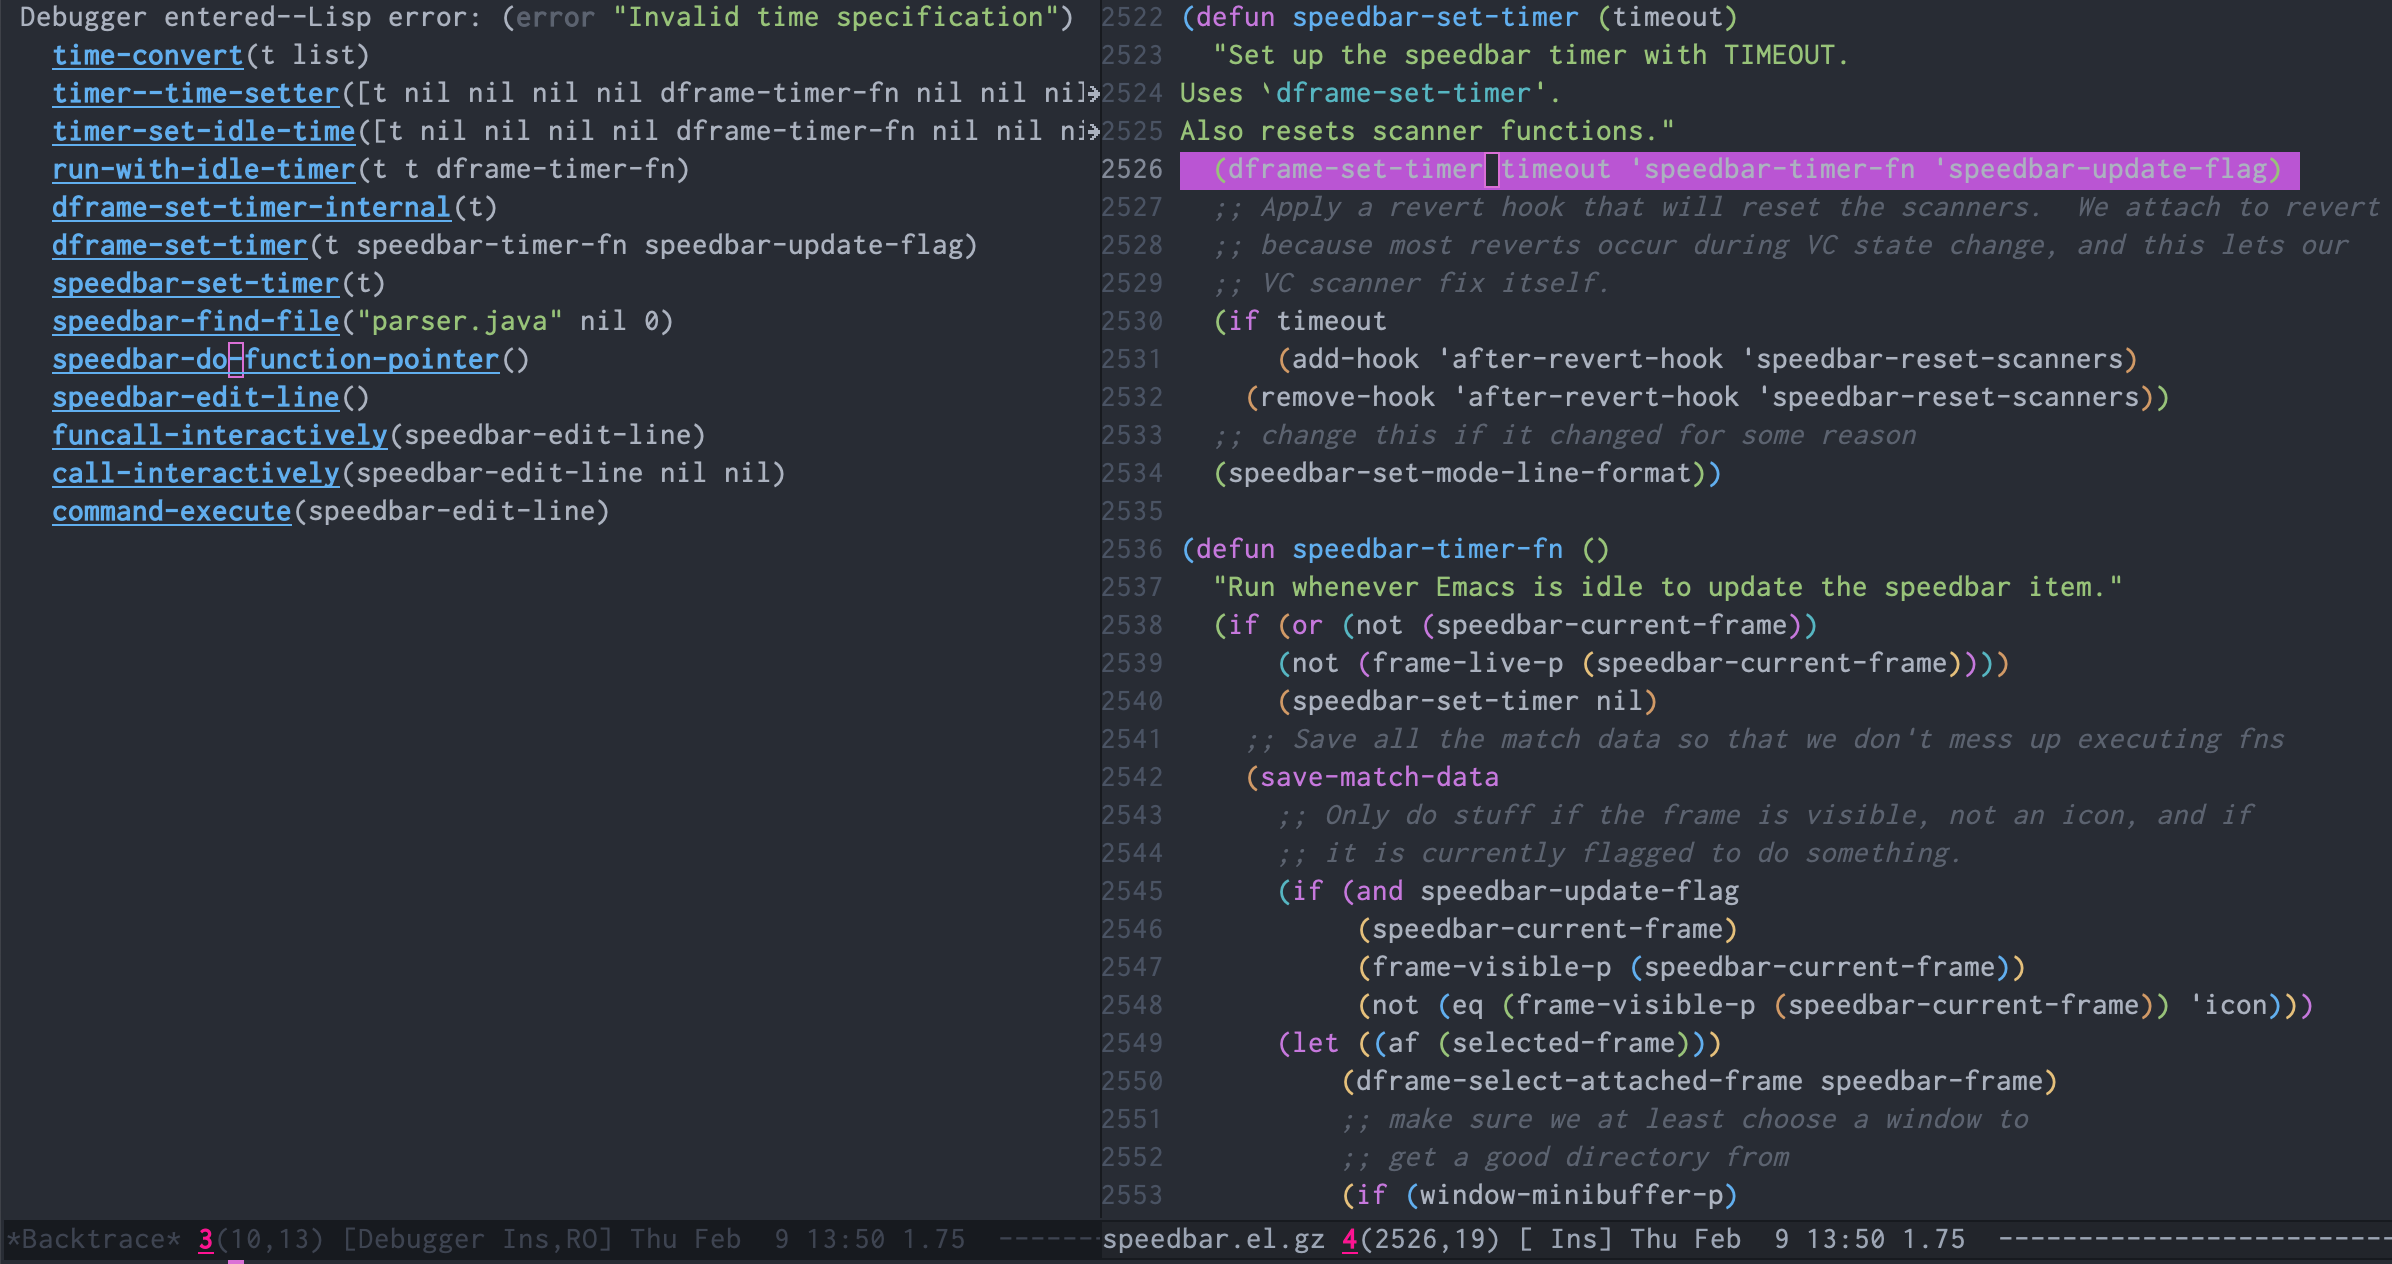
\includegraphics[width=.9\linewidth]{./pic/readme_20230209_135039.png}
\begin{itemize}
\item 好像是macOS系统常常存在的 bug,两年了关了又开,开了再关\ldots{}\ldots{}
\item \url{https://github.com/remacs/remacs/issues/845}
\item get cmake work later, not urgent though.Complete
\item babel org-mode so I don't have to copy from specific babeled source org-mode files in order for chinese characters to work.
\item Installed my emacs of version 28.1. But there is a bug of any verison emacs > 27.1, and I am NOT able to find a installable emacs 27.1 version any more.
\item 不同电脑架构上可能因为架构的不同,可以可能可以有某些优化.又照一个单做了一遍,似乎没有出错. \url{https://goykhman.ca/gene/blog/2022/2022-04-10-emacs-28.1-on-m1.html}
\item 但是我没有没能加入那个补丁包.暂时没能想好怎么加入那个补丁包. ( \textbf{todo: 改天可以尝试再把这个补丁包加进去} )
\item 因为构建是在原有现有的 mac 28.1.1版本上构建的.所以改动什么,或是不曾改变,又或者改不了不影响明显功能都是无从知晓的,但是它最后的两个步骤的验证都是成功的,应该还是构建成功了吧?
\end{itemize}

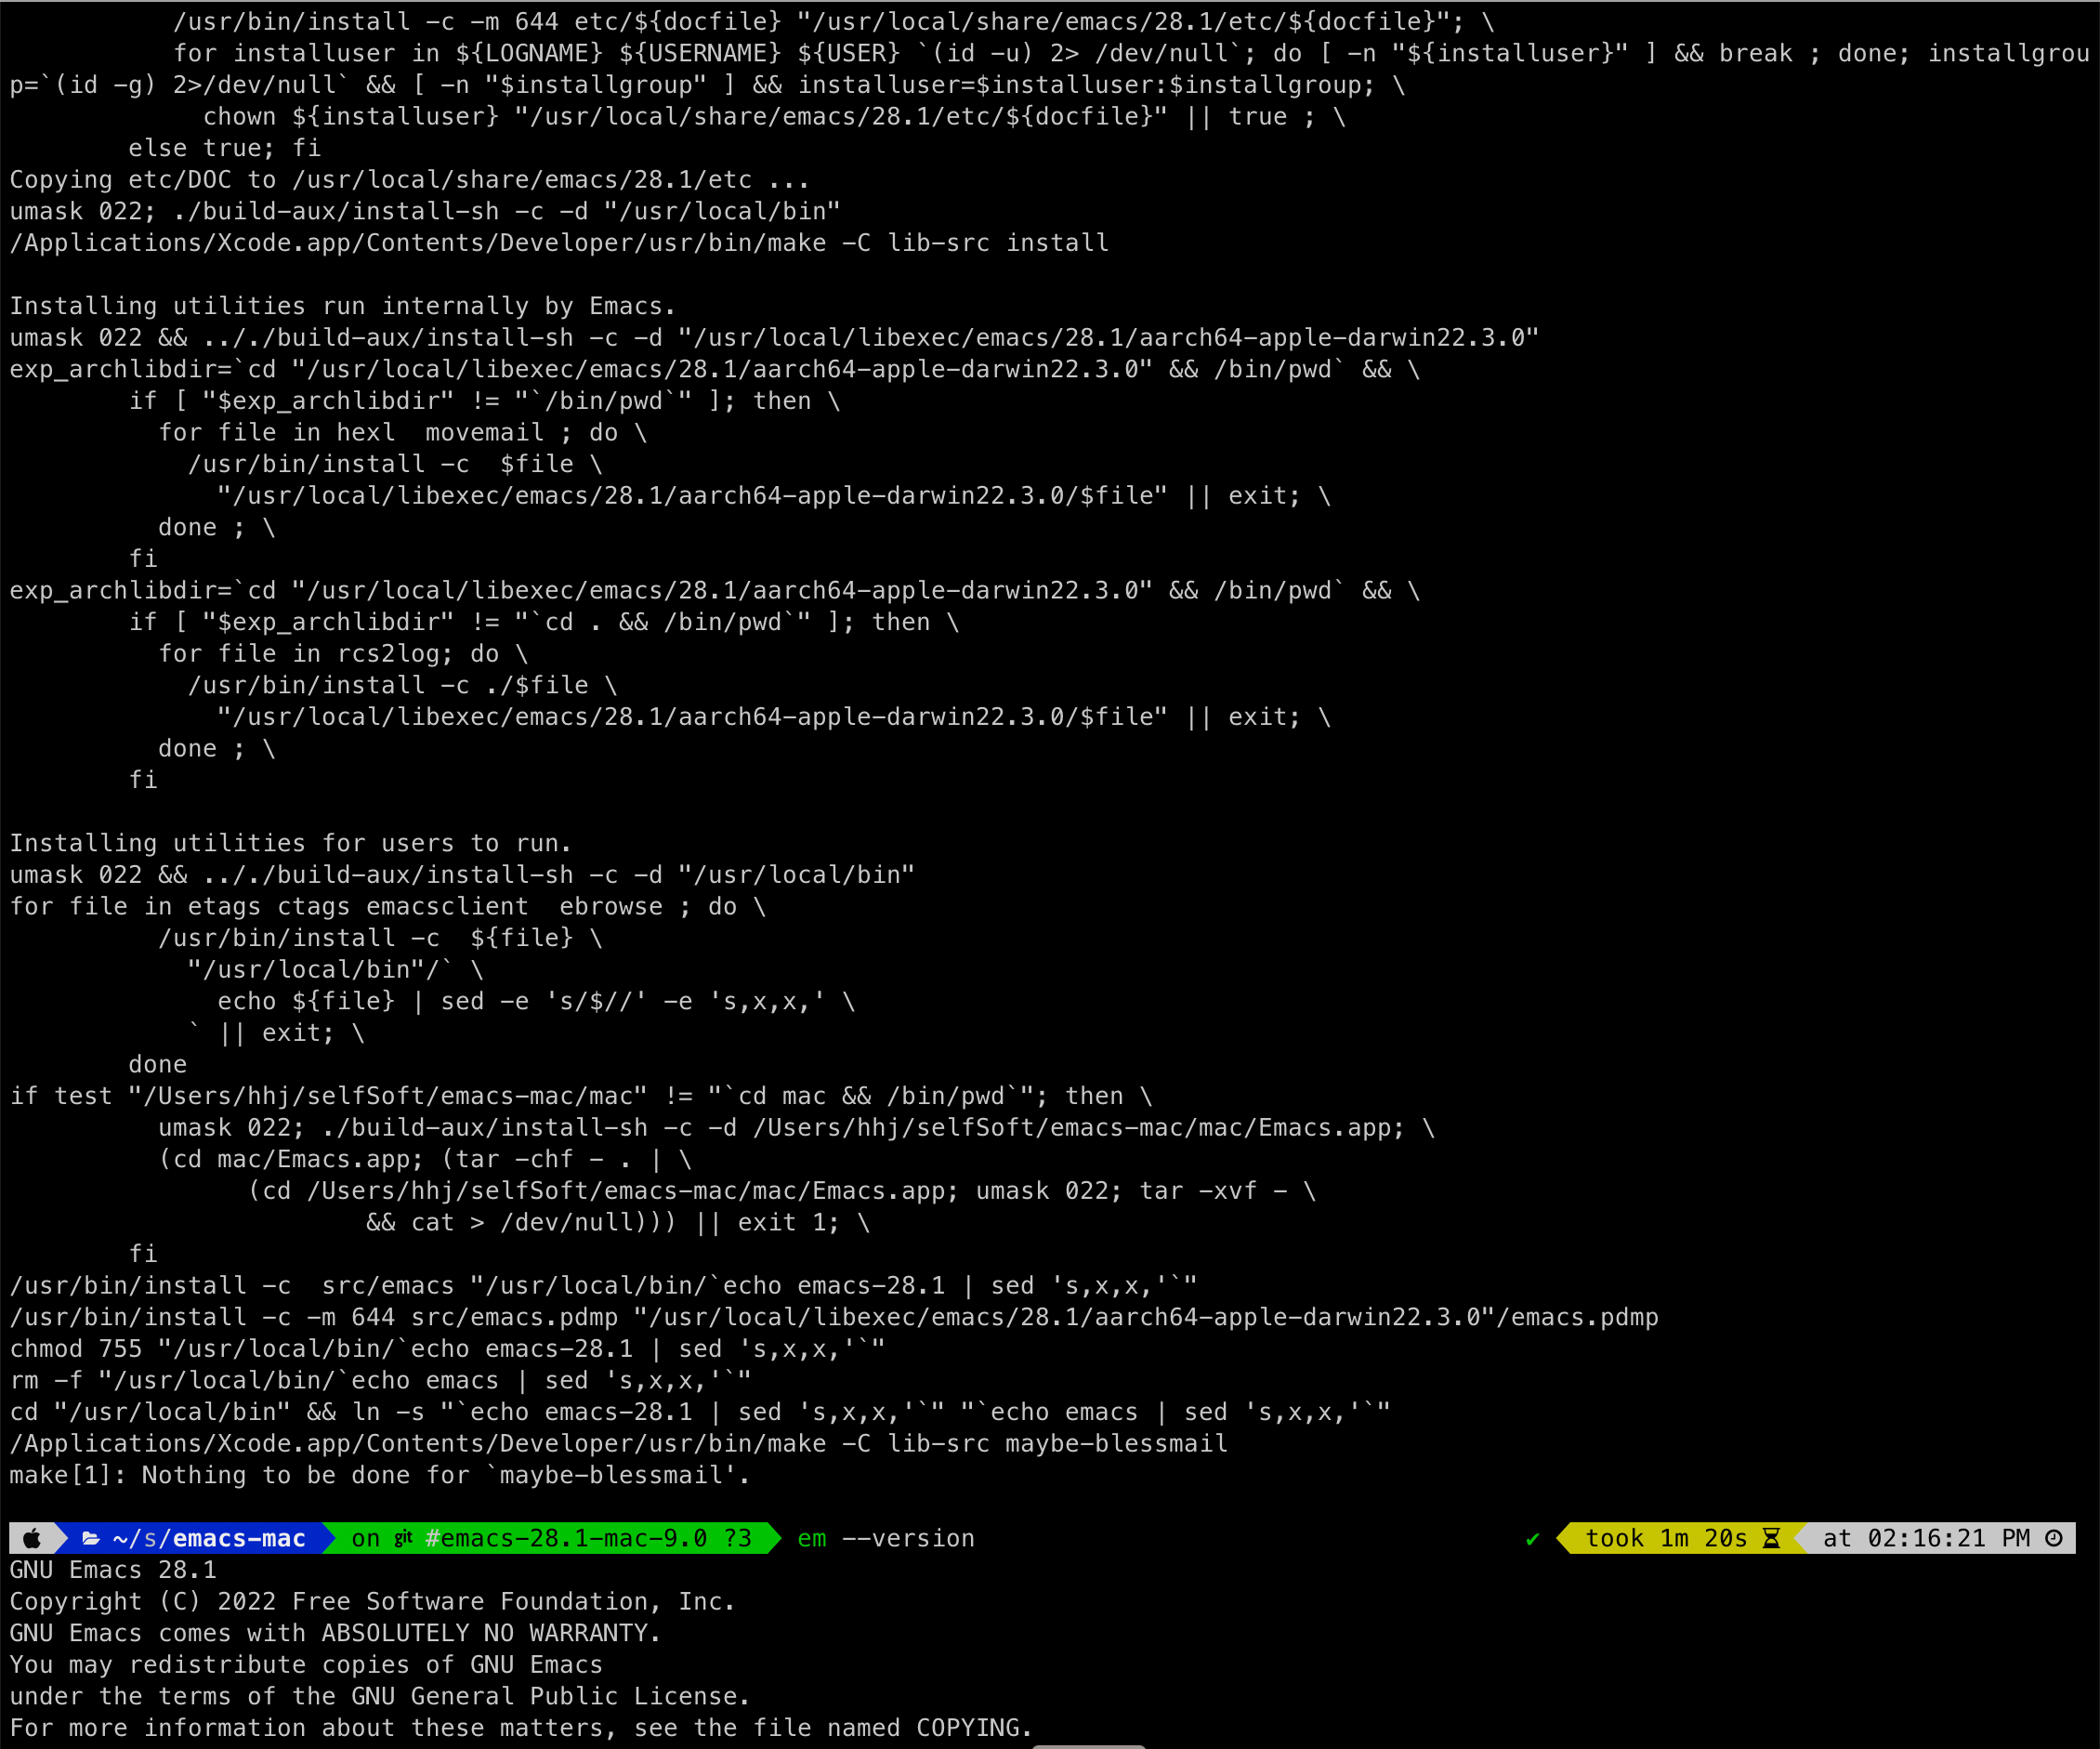
\includegraphics[width=.9\linewidth]{./pic/readme_20230208_142554.png}
\begin{itemize}
\item 今天又尝试安装Xcode之后再构建一遍,但是没有成功.可能本身参考有些年代,另外自己还完全不通这个部分,所以暂时放一放.改天有机会可以再回来研究一下,错在哪里,我如何才可能构建出自己的版本.
\end{itemize}

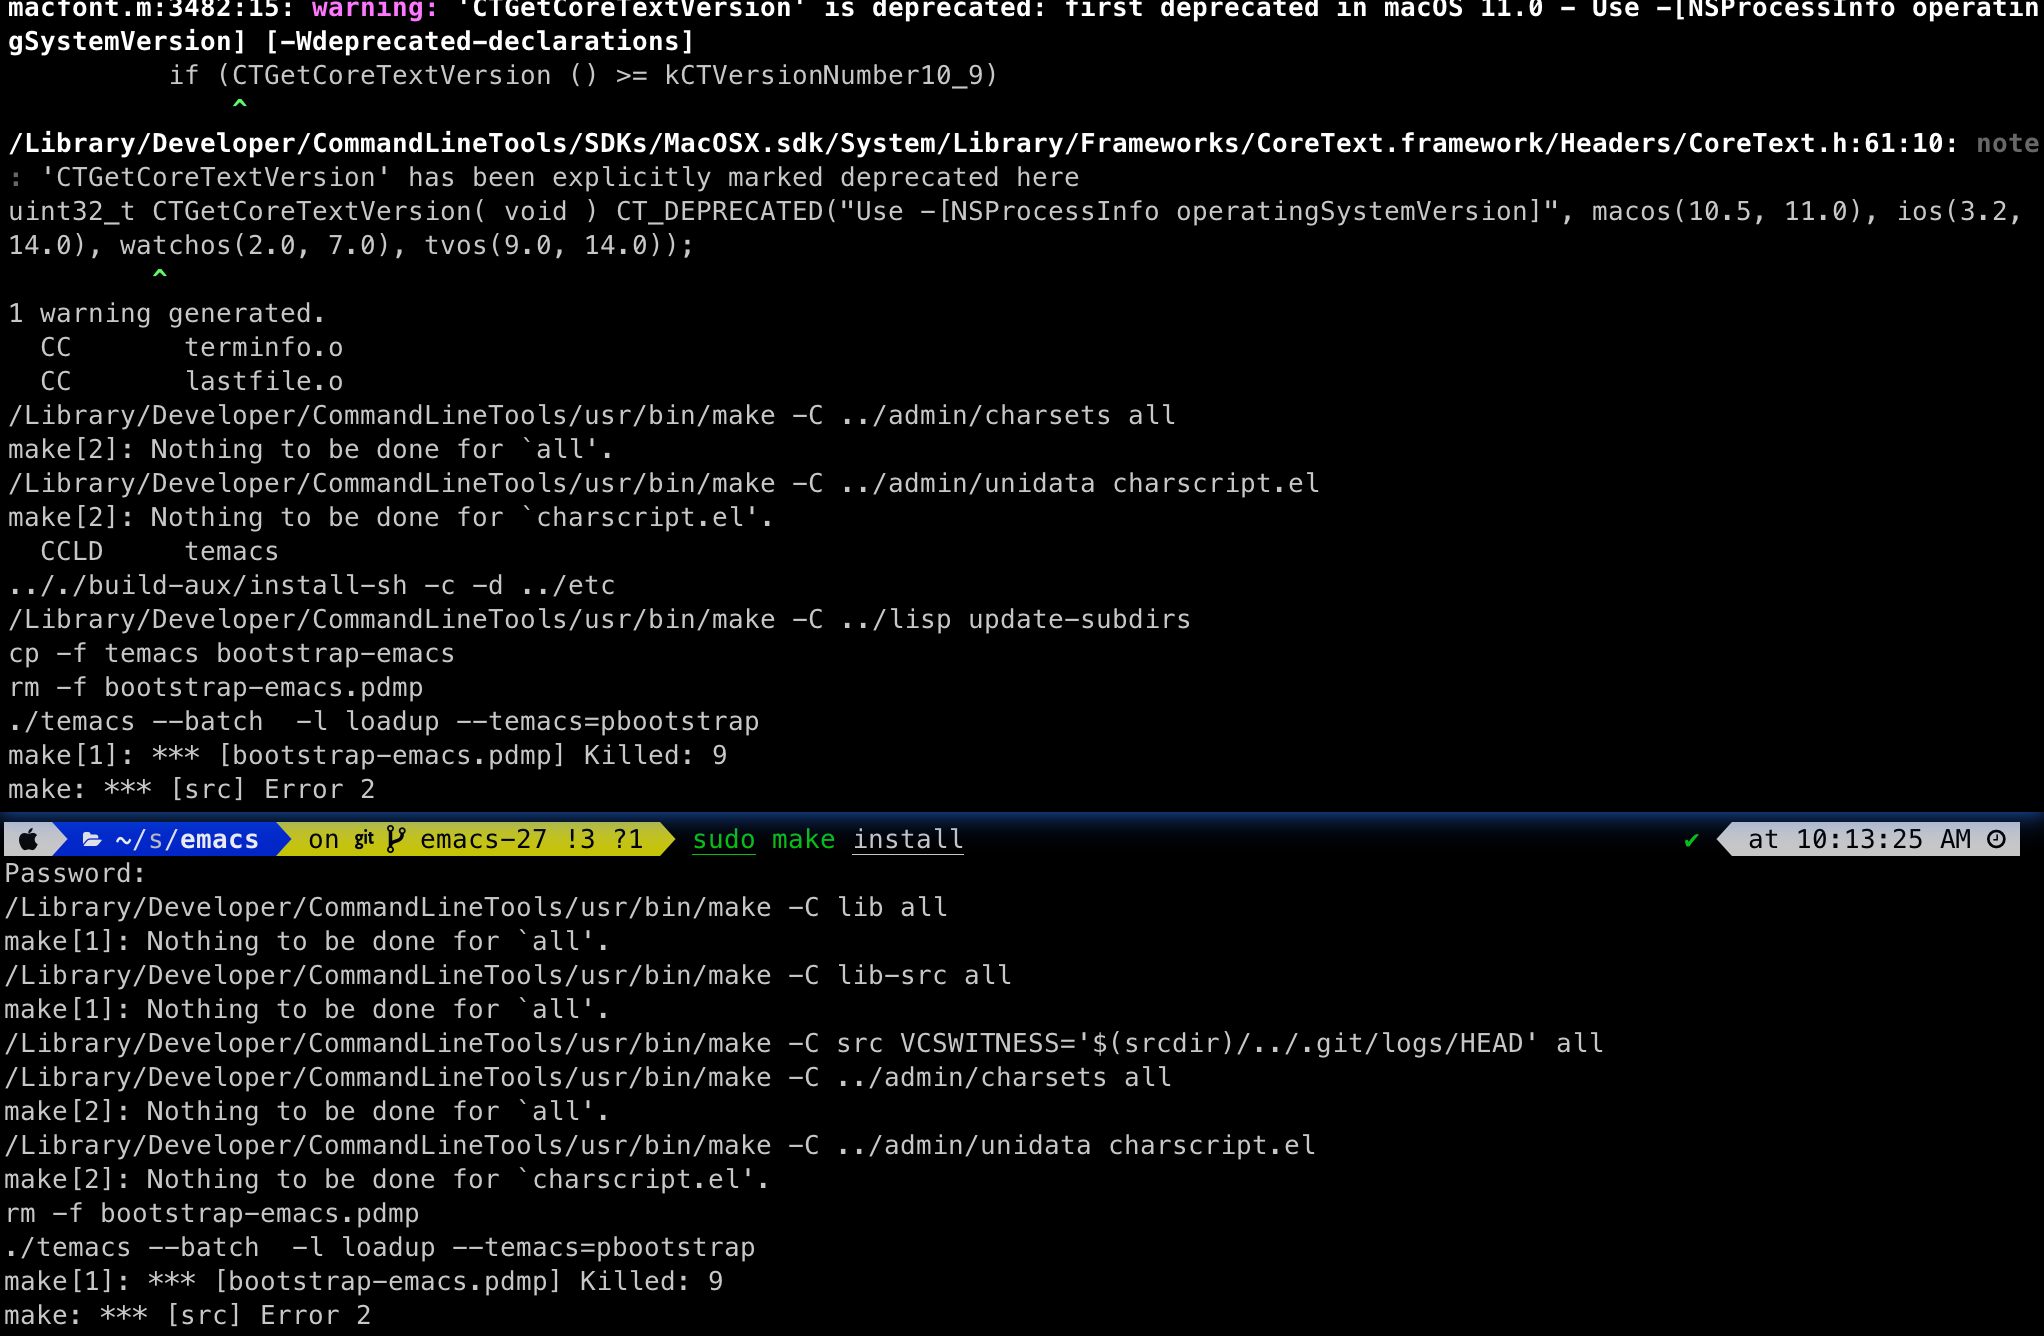
\includegraphics[width=.9\linewidth]{./pic/readme_20230208_102317.png}
\begin{itemize}
\item 上面又成为一个需要改的东西: 就是系统下如何从剪贴板自动生成写入文件 org-mode M-s
\item 然后看见这里说可以自己构建一个,连Xcode也没有安装,就跑去构建了,当然不成功。这段时间太忙,XCode要的空间太大了,暂时还不想。等改天有机会的时候倒是可以一试的
\begin{itemize}
\item \url{https://stuff-things.net/2020/12/28/building-emacs-27-dot-1-on-macos-big-sur/}
\end{itemize}
\item added key-bindings for opening from VSCode/Android Studio of current emacs buffer. 
\begin{itemize}
\item VSC Emacs can locate to each othr to correct row and col.
\item Android Studio could open current emacs buffer. but not to the row nor col.
\end{itemize}
\item I liked recently configued Visual studio 2019 one-dark-pro theme, want to configue it for emacs, but ended up with any permission denied, renaming emacs initiating bug. reverted back for daily use, and may look into that bug for later reference.
\item will reconfigure one-dark-pro theme later.
\item fixed legency java-mode highlighing issue which I did not fix for years. Has been able to treat java-mode as java-mode Instead of using it as csharp-mode. Can not separate java-mode snippets from csharp-mode's.
\end{itemize}
\subsection{BUG statement and partial fix}
\label{sec-1-5}
\begin{itemize}
\item in java-mode, the code style I expected is as followed:
\end{itemize}
\begin{minted}[fontsize=\scriptsize,linenos=false]{java}
class node {
    int v ;
    public node() {
        if (a > 0) // I don't want { } blocks when I have only one line statement inside blocks
     // a = 17;    // before fix:
            a = 17;   // now it can auto-indent
        b = 20;
        while (true)  // same auto indents here
            j++;
    }
}
class dklfjdj {|} // <<==== current un-auto-expanded version, bug right now for java-mode
class dklfjdj { 
    | // <<==== expected feature: once I typed '{', '}' will be autopaired(it does), but also auto-expand and cursor moves and indents directly to where I expect
}
\end{minted}
\begin{itemize}
\item if while if while one line statement autoindent without \{\} fixed today for java-mode, but for kotlin-mode, this bug consists, make coders/programmers nuts.
\end{itemize}
\begin{minted}[fontsize=\scriptsize,linenos=false]{java}
fun getStringLength(obj: Any): Int? {
    if (obj is String)
    return obj.length  // <<<<===== BUG: need to fix auto-indent here for if else while etc without {} 

    if (obj is String) {
        return obj.length
    }
    // 在离开类型检测分支后,`obj` 仍然是 `Any` 类型
    return null
}
fun dslfkj { // kotlin-mode, unlike java-mode, this feature works charming
    val a = 1720 
}
\end{minted}
\begin{itemize}
\item The \{|\} can NOT auto-expand still bugs me a lot, I don't want to switch back to java-mode yet unless bug fixed and it auto-pands.
\item java minor bug: Debugger entered--Lisp error: (void-function company-clear-completion-rules): this bug I will look into it recently, and expect it to be fixed so I could switch java-mode from csharp-mode as soon as possible.
\item \textbf{csharp-mode} has been the one that works perfectly for these two features, \{\} auto expand, also if while one line statement autoindent without \{\}, so I used csharp-mode as java mode.
\end{itemize}
\section{References}
\label{sec-2}
\begin{itemize}
\item \url{https://github.com/redguardtoo/emacs.d}
\end{itemize}
% Emacs 27.1 (Org mode 8.2.7c)
\end{document}